\begin{figure}[tb]
\centering
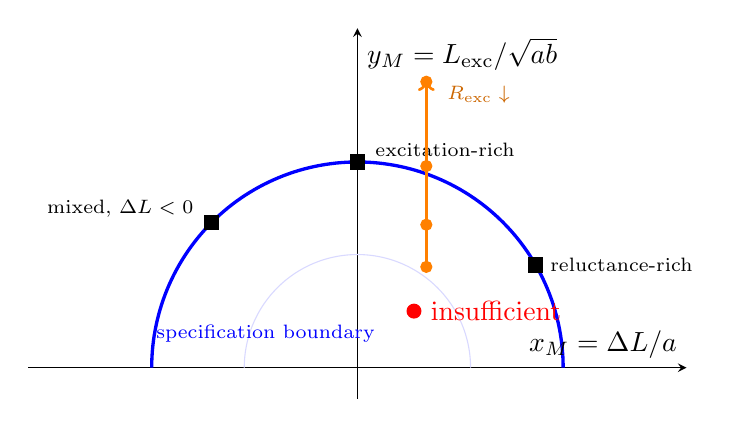
\begin{tikzpicture}
\begin{axis}[
 width=.82\linewidth,height=.55\linewidth,
 axis equal image,axis lines=middle,xmin=-3.2,xmax=3.2,ymin=-.3,ymax=3.3,
 xlabel={$x_M=\Delta L/a$},ylabel={$y_M=L_{\mathrm{exc}}/\sqrt{ab}$},
 ticks=none,clip=false]
 \addplot[domain=0:180,samples=121,blue,very thick]
   ({2*cos(x)},{2*sin(x)});
 \addplot[blue!15,domain=0:180,samples=121] ({1.1*cos(x)},{1.1*sin(x)});
 \addplot[only marks,mark=*,mark size=2.5pt,red] coordinates {(.55,.55)};
 \node[red,anchor=west] at (axis cs:.62,.55) {insufficient};
 \addplot[only marks,mark=square*,mark size=2.6pt,black]
   coordinates {(1.73,1) (0,2) (-1.42,1.41)};
 \node[anchor=west,font=\scriptsize] at (axis cs:1.78,1) {reluctance-rich};
 \node[anchor=west,font=\scriptsize] at (axis cs:.08,2.12) {excitation-rich};
 \node[anchor=east,font=\scriptsize] at (axis cs:-1.5,1.55) {mixed, $\Delta L<0$};
 \addplot[orange,very thick,->] coordinates {(.67,.98) (.67,1.39) (.67,1.96) (.67,2.78)};
 \addplot[only marks,orange,mark=*] coordinates {(.67,.98) (.67,1.39) (.67,1.96) (.67,2.78)};
 \node[orange!80!black,anchor=west,font=\scriptsize] at (axis cs:.78,2.65)
   {$R_{\mathrm{exc}}\downarrow$};
 \node[blue,anchor=south west,font=\scriptsize] at (axis cs:-2.05,.15)
   {specification boundary};
\end{axis}
\end{tikzpicture}
\caption{Loss-limited EESM capability map.  Constant torque per copper loss
forms circles.  Points on one circle have equal scalar capability but different
physical mechanisms.  The orange synthetic sweep shows the false divergence
created when excitation resistance is driven toward zero without adding a
replacement field constraint.}
\label{fig:machine-capability}
\end{figure}

